\chapter{Introduction To Groups}
In this chapter, we motivate the definition and use of groups in mathematics.

\section{The Study of Symmetry}
A group is a \textit{collection of symmetries of something}. A symmetry is a \textit{mapping} from something to itself that \textit{preserves structure}. This is, of course, not the formal definition of a group, but it gives an intuition of \textit{why} mathematicians care about groups.

\begin{wrapfigure}{r}{0.35\textwidth}
    \centering
    \fbox{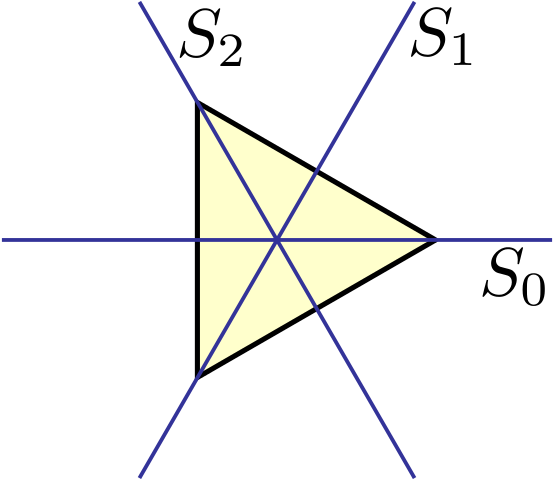
\includegraphics[width=0.3\textwidth]{intro-to-groups/triangle-reflections.png}}
\end{wrapfigure}

For example, one may consider the collection of symmetries of an equilateral triangle. What actions could one perform to make the triangle ``look the same'' as before applying the action? Well, we could do nothing. That action is called the \textit{identity action}. We could also reflect the triangle about the line $S_0$ and observe that the triangle ``looks the same as before''. We may also reflect the triangle about the lines $S_1$ and $S_2$, and the triangle will still ``look the same as before''. One may also consider rotating the triangle $120^\circ$ or $240^\circ$ about the centre in a clockwise manner (note that rotating the triangle $360^\circ$ is the same as the identity action, so we do not count it here).

So we count 6 distinct actions in total: 1 identity action, 2 rotation actions, and 3 reflection actions. We can say that the \textit{group of symmetries of the equilateral triangle} has 6 actions (or elements) in total.

\begin{wrapfigure}{r}{0.35\textwidth}
    \centering
    \fbox{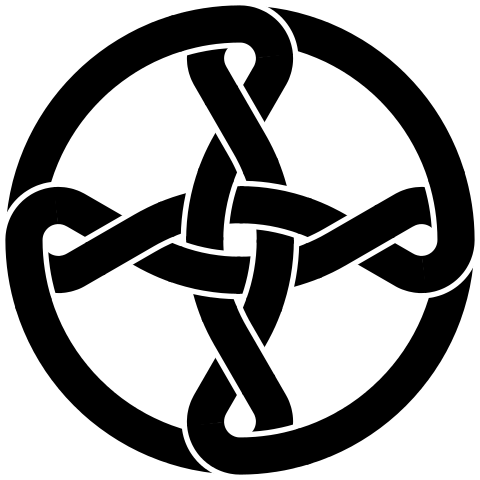
\includegraphics[width=0.3\textwidth]{intro-to-groups/circular-crossings.png}}
\end{wrapfigure}

Another category of groups that we can consider is \textit{groups of rotation}. For example, consider the image on the right. There are 4 actions that we can do to this image that makes it ``look the same as before''.
\begin{itemize}
    \item Do nothing (the identity action).
    \item Rotate the circle $90^\circ$ clockwise.
    \item Rotate the circle $180^\circ$ clockwise.
    \item Rotate the circle $270^\circ$ clockwise.
\end{itemize}
Note that the image has \textbf{no} lines of symmetry; due to the unique braiding on the knots, this image only has \textit{rotational symmetry} and no \textit{mirror} (or \textit{reflective}) \textit{symmetry}. Thus, this group has only 4 actions, all of which are rotations. One could say that this group is a \textit{cyclic group} and that it has \textit{order} 4. We'll formally define what these terms mean in later chapters.

\begin{wrapfigure}{r}{0.4\textwidth}
    \centering
    \fbox{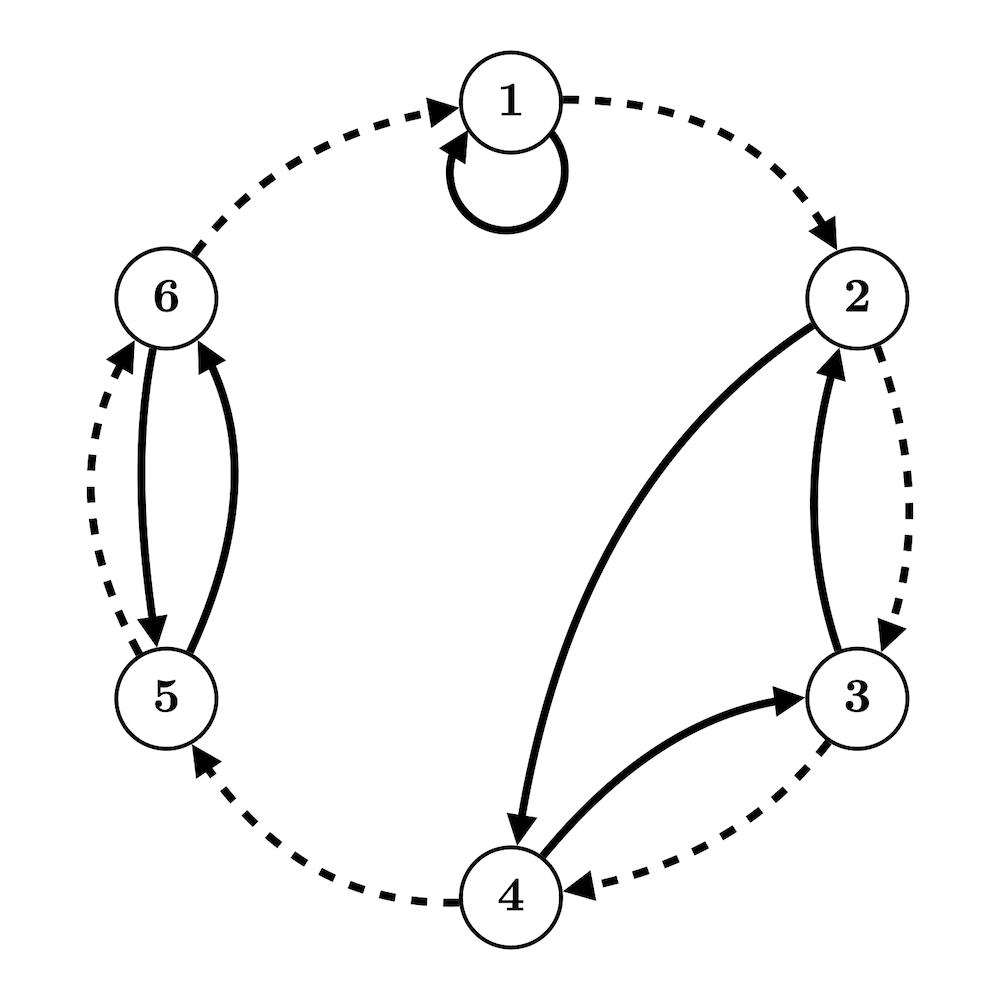
\includegraphics[width=0.35\textwidth]{intro-to-groups/permutations.png}}
\end{wrapfigure}

Let's look at a more technical example. Consider a set of points in a pane. We can consider the \textit{group of symmetries of a finite collection of points}. What are the symmetries of the points? Well, in this case, a \textit{symmetry} is a way to move one of these points to another point while making it ``look the same as before''.

\begin{itemize}
    \item One possible symmetry is given by the solid arrows. In such a symmetry, we have a a point (1) mapping to itself, a cycle of 2 points (5 and 6) on the left, and a cycle of 3 points (2, 3, and 4) on the right. Since the points ``look the same as before'', this is a valid symmetry.
    \item Another possible symmetry is given by the dotted arrows. In this case, all points are shifted clockwise in a circle. Since the points ``look the same as before'', this is valid.
\end{itemize}

One may notice that what each of the symmetries is doing is \textit{permuting} the points around. In this case, this is exactly what each of the symmetries is doing: generating a possible permutation of points and ensuring that their locations stay the same. The collection of symmetries is thus called the \textit{symmetric group of degree 6}, and its group actions compose of \textit{bijections from the set to itself}.

\begin{exercise}
    How many symmetries are there in the symmetric group of degree 6? In other words, what is the order of the group above?\newline
    (\textit{Hint: Consider the number of permutations in the group.})
\end{exercise}

\section{What Constitutes a Group?}
Now that we have taken a look at some examples of groups, we ask: what properties do all groups satisfy? These properties are called the \textbf{group axioms}. We motivate the `discovery' of each axiom with examples.

\begin{wrapfigure}{r}{0.325\textwidth}
    \centering
    \fbox{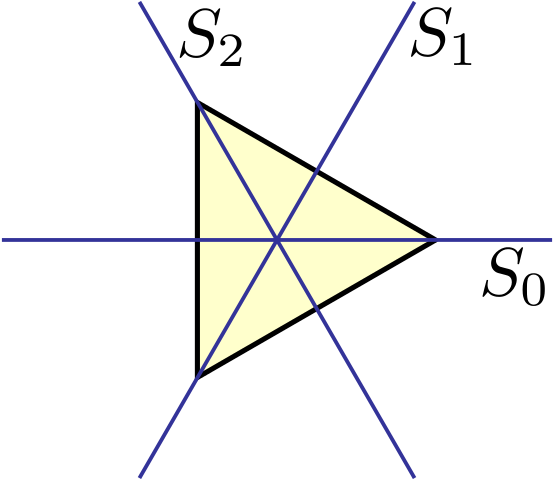
\includegraphics[width=0.275\textwidth]{intro-to-groups/triangle-reflections.png}}
\end{wrapfigure}

Consider the group of symmetries of an equilateral triangle. One condition that that group must satisfy is that performing group actions one after another should not make the underlying object ``non-symmetric''. We should not be able to form a group action that results in the triangle being ``non-symmetric''. For example, we do not include rotating the triangle $90^\circ$ clockwise about $S_0$ (into 3D space) as this immediately makes the triangle ``different to how it began''.

This property can be called the \textbf{axiom of closure} and can be written like this:
\begin{quote}
    A group $(G, \ast)$ is a set $G$ together with a binary operation $\ast$ that ensures closure. That is, if $a$ and $b$ are in $G$, then $a \ast b$ is also in $G$.
\end{quote}
(Of course, this is not the actual definition, but we'll get into it later.)

The set $G$ in the previous example is the set of actions on the equilateral triangle that preserves symmetry. The binary operation $\ast$ can be informally called the ``followed by'' operator. Thus
\begin{quote}
    (reflect about $S_0$) $\ast$ (rotate the triangle 120° clockwise)
\end{quote}
means
\begin{quote}
    rotate the triangle 120° clockwise, \textit{followed by} reflection about $S_0$
\end{quote}
in standard English. It should be noted that we read actions \textbf{from right to left}, as seen in the example above. In the following chapters, such actions will be replaced with symbols.

Another property that a group must have is that it must contain an \textit{identity element}. We emphasised this property numerous times in the previous examples. This is called the \textbf{axiom of identity} and is phrased as follows.
\begin{quote}
    A group $(G, \ast)$ has an element $e$ where, for any element $x$ in the group, it satisfies $e \ast x = x \ast e = x$.
\end{quote}
This means that the identity action should do nothing. Applying the action before or after another action should just perform the action.

We would also like, for every action, to have an action that \textit{undoes} the previous action. For example, for rotation, we would like to have an action that undoes the rotation. This action is called the \textit{inverse} of the action, and the \textbf{axiom of inverse} guarantees that every action in a group has an inverse.

\begin{quote}
    For every element $x$ in the group $(G, \ast)$, there exists an action in the group, called the inverse of $x$ and denoted by $x^{-1}$, such that $x \ast x^{-1} = x^{-1} \ast x = e$.
\end{quote}

\begin{wrapfigure}{r}{0.35\textwidth}
    \centering
    \fbox{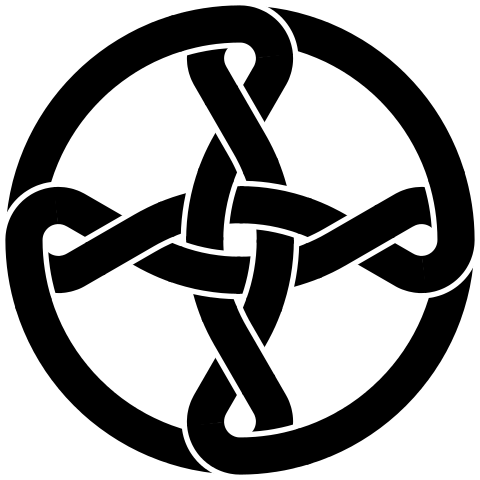
\includegraphics[width=0.3\textwidth]{intro-to-groups/circular-crossings.png}}
\end{wrapfigure}

The last axiom is hard to discover naturally and hard to motivate, but is absolutely necessary for groups. Consider again this braided circle, and let's say we want to perform 3 rotations (say, $r_1$, $r_2$ and $r_3$) in that sequence. We would not want to distinguish between performing ``$r_1$, then $r_2$ and $r_3$'' (i.e., $r_1 \ast (r_2 \ast r_3)$), and ``$r_1$ then $r_2$, then $r_3$'' (i.e. $(r_1 \ast r_2) \ast r_3$). We are only concerned about the \textit{sequence} of the rotations. This is called the \textbf{axiom of associativity}:
\begin{quote}
    Let $x, y$, and $z$ be elements in $(G, \ast)$. Then $(x \ast y) \ast z = x \ast (y \ast z)$.
\end{quote}

\newpage

So what is a group?
\begin{definition}
    A \textbf{group}\index{group} is a set $G$ together with a operation on $G$, here denoted by $\ast$, satisfying the following axioms.
    \begin{enumerate}
        \item \textbf{Closure}\index{axiom!of closure}: For all elements $a$ and $b$ in $G$, $a \ast b$ is also in $G$.
        \item \textbf{Associativity}\index{axiom!of associativity}: For all elements $a, b$, and $c$ in $G$, we have $a \ast (b \ast c) = (a \ast b) \ast c$.
        \item \textbf{Identity}\index{axiom!of identity}: There exists an element $e$ in $G$ such that for any element $x$ in $G$ we have $e \ast x = x \ast e = x$.
        \item \textbf{Inverse}\index{axiom!of inverse}: For every element $x$ in $G$, there exists an element $x^{-1}$ in $G$ such that $x \ast x^{-1} = x^{-1} \ast x = e$.
    \end{enumerate}
\end{definition}

Usually, for the brevity of notation, we will write $a \ast b$ as $ab$. We will look at more properties of groups in later chapters. We would usually suppress the operation $\ast$ when defining a group, so instead of saying that the group is $(G, \ast)$, we just say that the group is $G$.

We will look at examples of groups in the next chapter.

\newpage

\section{Problems}
\begin{problem}
Determine whether the following are groups. If they are, prove it. If not, explain why they are not groups.
\begin{partquestions}{\alph*}
    \item $(\Z, +)$.
    \item $(\Z \setminus \{0\}, \times)$ where $\times$ denotes regular multiplication.
    \item $(\R \setminus \{0\}, \times)$ where $\times$ denotes regular multiplication.
    \item $(\{0\}, \times)$ where $\times$ denotes regular multiplication.
    \item $(\{1\}, +)$ where $+$ denotes regular addition.
    \item $(\{1\}, \times)$ where $\times$ denotes regular multiplication.
\end{partquestions}
\end{problem}

\begin{problem}
    Show that the \textbf{trivial group}\index{trivial group} $(\{e\}, *)$ where $e \ast e = e$ is indeed a group.
\end{problem}
